\newpage


\subsubsection{UCA 3 - Gestione lista delle organizzazioni}%kite level
\begin{figure}[h]
	\centering
	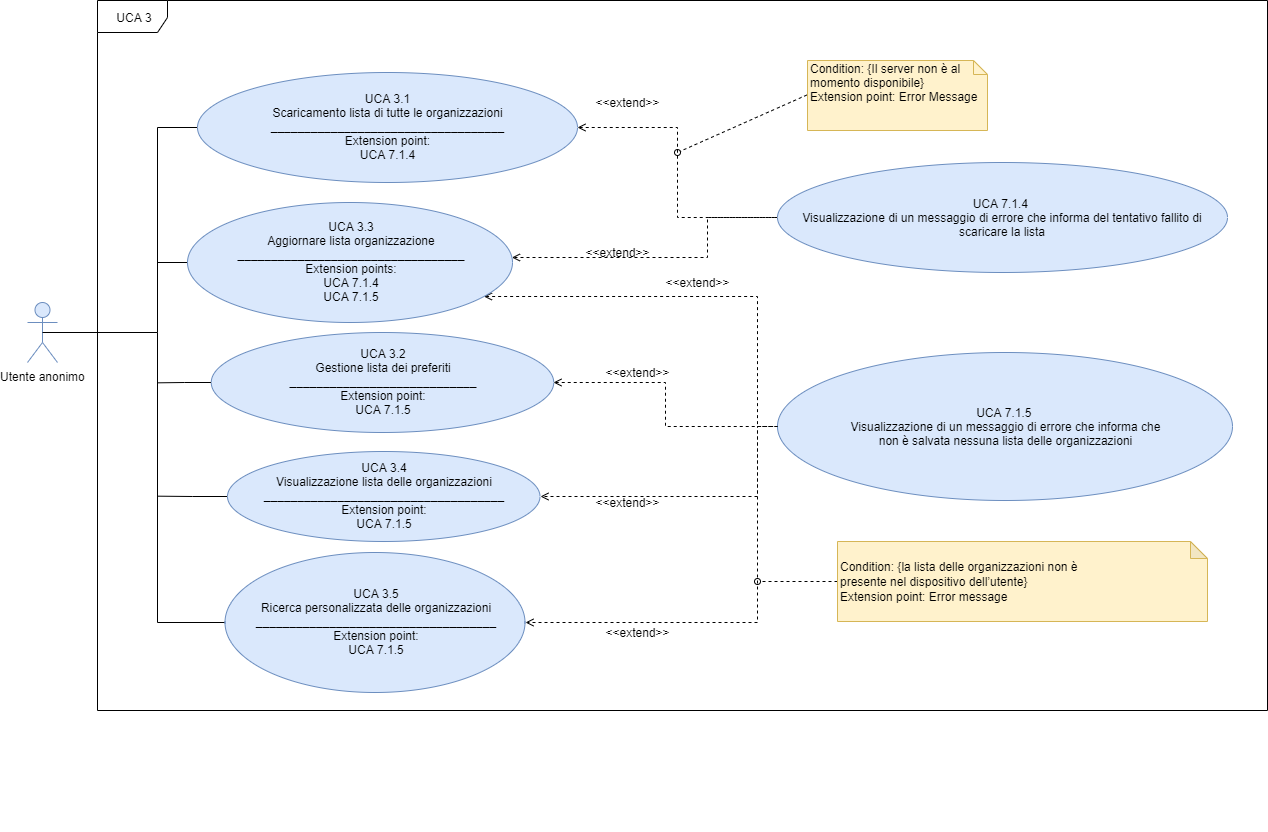
\includegraphics[scale=0.33]{sezioni/UseCase/Immagini/UCA3.png}
	\caption{UCA 3 - Gestione lista delle organizzazioni}
\end{figure}

\begin{itemize}
\item \textbf{Attori primari:} Utente anonimo;
\item \textbf{Precondizione:} L'utente è autenticato e può accedere alle funzionalità della lista delle organizzazioni;
\item \textbf{Postcondizione:} Vengono forniti all'utente i risultati delle funzionalità disponibili;
\item \textbf{Scenario principale:} L'utente autenticato utilizza le funzioni di gestione delle liste di organizzazioni per svolgere le diverse azioni;
\item \textbf{Flusso di eventi:}
	\begin{itemize}
		\item UCA 3.1 - Scaricamento lista di tutte le organizzazioni;
		\item UCA 3.2 - Gestione lista dei preferiti;
		\item UCA 3.3 - Aggiornare lista organizzazione;
		\item UCA 3.4 - Visualizzazione lista;
		\item UCA 3.5 - Ricerca personalizzata delle organizzazioni.
	\end{itemize}
\end{itemize}



\subsubsection{UCA 3.1 - Scaricamento lista di tutte le organizzazioni}%sea level
\begin{itemize}
\item \textbf{Attori primari:} Utente anonimo;
\item \textbf{Precondizione:} L'utente è autenticato e può scaricare la lista di tutte le organizzazioni;
\item \textbf{Postcondizione:} L'utente ha a disposizione la lista di tutte le organizzazioni;
\item \textbf{Scenario principale:} L'utente seleziona l'esecuzione della funzione "Scaricamento della lista";
\item \textbf{Scenario alternativo:}  Se il tentativo di scaricare la lista fallisce viene visualizzato all'utente un messaggio di errore che lo informa di tale problema;
\item \textbf{Estensioni:}
	\begin{enumerate}
	\item UCA 3.1.1 - Visualizzazione di un messaggio di errore che informa del tentativo fallito di scaricare la lista.
\end{enumerate}
  
\end{itemize}

\subsubsection{UCA 3.1.1 - Visualizzazione di un messaggio di errore che informa del tentativo fallito di scaricare la lista}%fish level
\begin{itemize}
\item \textbf{Attori primari:} Utente anonimo;
\item \textbf{Precondizione:} L'utente esegue l'azione di scaricare la lista delle organizzazioni ma fallisce;
\item \textbf{Postcondizione:} Viene visualizzato un messaggio d'errore che informa la non disponibilità del server.

\end{itemize}



\subsubsection{UCA 3.2 - Gestione lista dei preferiti}%sea level

\begin{figure}[h]
	\centering
	
	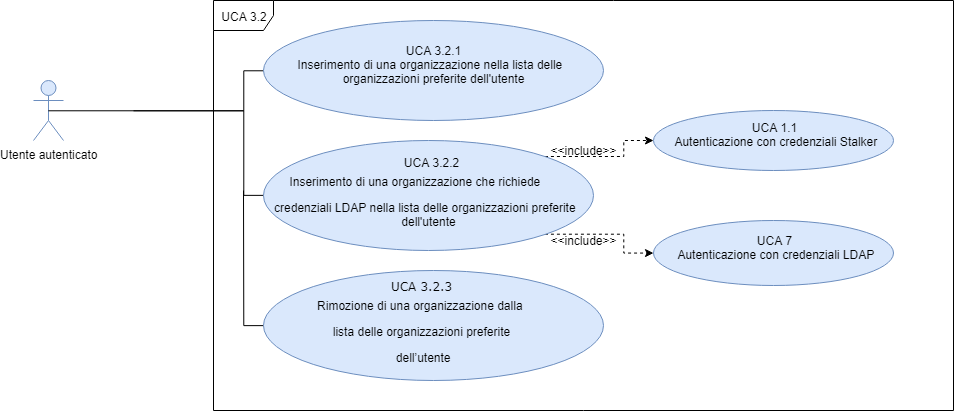
\includegraphics[scale=0.5]{sezioni/UseCase/Immagini/UCA3.2.png}
	\caption{UCA 3.2 - Gestione lista dei preferiti}
\end{figure}

\begin{itemize}
	\item \textbf{Attori primari:} Utente anonimo;
	\item \textbf{Precondizione:} L'utente è autenticato e può gestire la lista dei preferiti;
	\item \textbf{Postcondizione:} All'utente vengono fornite i risultati delle funzionalità disponibili;
	\item \textbf{Scenario principale:} L'utente autenticato ha selezionato la funzionalità di gestione della lista dei preferiti;
	\item \textbf{Flusso di eventi:}
			\begin{itemize}
			%\item L'utente accede alla funzionalità di "Gestioni della lista dei preferiti";
			\item UCA 3.2.1 - Inserimento di una organizzazione nella lista dei preferiti dell'utente dell'applicazione;
			\item UCA 3.2.2 - Rimozione di una organizzazione dalla lista dei preferiti dell'utente dell'applicazione;
			\end{itemize}
	\item \textbf{Scenario alternativo:} Se non è presente nessuna lista delle organizzazioni viene visualizzato all'utente un messaggio di errore che lo informa di tale problema;
	\item \textbf{Estensioni:}
	\begin{enumerate}
		\item UCA 3.3.3 - Visualizzazione di un messaggio di errore che informa che non è salvata nessuna lista delle organizzazioni.
	\end{enumerate}
\end{itemize}

\subsubsection{UCA 3.2.1 - Inserimento di una organizzazione nella lista dei preferiti dell'utente dell'applicazione}%fish level
\begin{itemize}
	\item \textbf{Attori primari:} Utente anonimo;
	\item \textbf{Precondizione:} L'utente anonimo sceglie di eseguire la funzionalità di inserimento nella lista dei preferiti; 
	\item \textbf{Postcondizione:} Viene inserita un'organizzazione scelta dall'utente, nella lista dei preferiti.
\end{itemize}

\subsubsection{UCA 3.2.2 - Rimozione di una organizzazione dalla lista dei preferiti dell'utente dell'applicazione}%fish level
\begin{itemize}
	\item \textbf{Attori primari:} Utente anonimo;
	\item \textbf{Precondizione:}  L'utente anonimo sceglie di eseguire la funzionalità di rimozione nella lista dei preferiti;
	\item \textbf{Postcondizione:} Viene rimossa un'organizzazione scelta dall'utente, dalla lista dei preferiti.
\end{itemize}



\subsubsection{UCA 3.3 - Aggiornare lista organizzazione}%sea level

\begin{figure}[h]
	\centering
	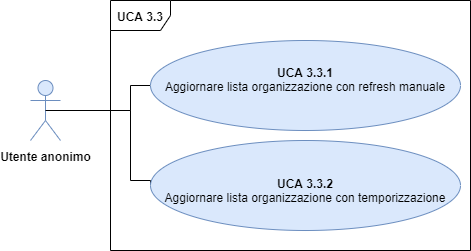
\includegraphics[scale=0.5]{sezioni/UseCase/Immagini/UCA3.3.png}
	\caption{UCA 3.3 - Aggiornare lista organizzazione}
\end{figure}

\begin{itemize} 
	\item \textbf{Attori primari:} Utente anonimo;
	\item \textbf{Precondizione:} L'utente è autenticato e può aggiornare la lista delle organizzazioni;
	\item \textbf{Postcondizione:} L'utente ha aggiornato la lista di tutte le organizzazioni;
	\item \textbf{Scenario principale:}  L'utente ha la necessità di aggiornare la lista e può farlo in diversi modi;
	\item \textbf{Flusso di eventi:}
	\begin{itemize}
		\item UCA 3.3.1 Aggiornamento lista organizzazione con refresh manuale;
		\item UCA 3.3.2 Aggiornamento lista organizzazione con temporizzazione;
	\end{itemize}
	\item \textbf{Scenario alternativo:} Se il tentativo di scaricare la lista falisce viene visualizzato all'utente un messaggio di errore che lo informa di tale problema. Se non è presente nessuna lista delle organizzazioni viene visualizzato all'utente un messaggio di errore che lo informa di tale problema;
	\item \textbf{Estensioni:}
	\begin{enumerate}
		\item UCA 3.1.2 Visualizzazione di un messaggio di errore che informa del tentativo fallito di scaricare la lista.
		\item UCA 3.3.3 Visualizzazione di un messaggio di errore che informa che non è salvata nessuna lista delle organizzazioni
	\end{enumerate}
\end{itemize}

\subsubsection{UCA 3.3.1 - Aggiornare lista organizzazione con refresh manuale}%fish level
\begin{itemize}
	\item \textbf{Attori primari:} Utente anonimo;
	\item \textbf{Precondizione:} L'utente anonimo sceglie di eseguire la funzionalità aggiornamento della lista dell'organizzazione attraverso la modalità di refresh manuale;
	\item \textbf{Postcondizione:} Viene eseguito l'aggiornamento della lista delle organizzazioni attraverso un refresh manuale.
	
\end{itemize}

\subsubsection{UCA 3.3.2 - Aggiornare lista organizzazione con temporizzazione}%fish level
\begin{itemize} 
	\item \textbf{Attori primari:} Utente anonimo;
	\item \textbf{Precondizione:} L'utente anonimo sceglie di eseguire la funzionalità aggiornamento della lista dell'organizzazione attraverso la modalità temporizzazione; 	
	\item \textbf{Postcondizione:} Viene eseguito l'aggiornamento della lista dell'organizzazione attraverso la modalità temporizzazione.
\end{itemize}

\subsubsection{UCA 3.3.3 - Visualizzazione di un messaggio di errore che informa che non è salvata nessuna lista delle organizzazioni}%fish level
\begin{itemize}
	\item \textbf{Attori primari:} Utente anonimo;
	\item \textbf{Precondizione:} La lista delle organizzazioni non è presente nel dispositivo dell'utente;
	\item \textbf{Postcondizione:} Viene visualizzato un messaggio di errore che informa che nel dispositivo non è presente la lista delle organizzazioni.
\end{itemize}

\newpage


\subsubsection{UCA 3.4 - Visualizzazione lista}%sea level

\begin{figure}[h]
	\centering	
	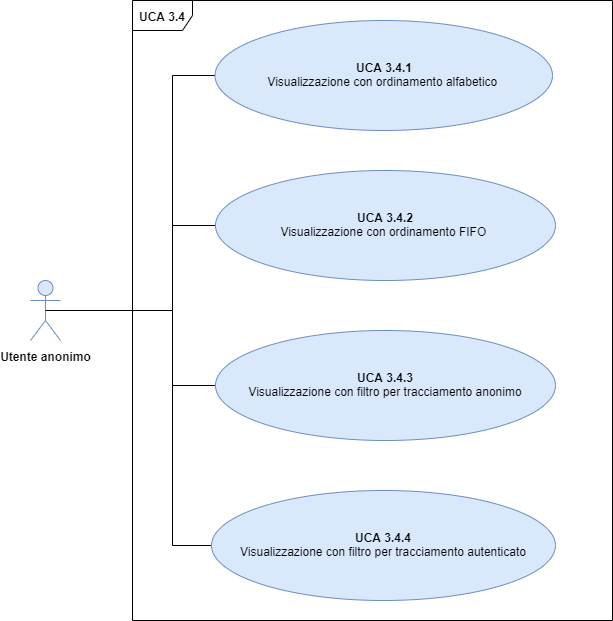
\includegraphics[scale=0.5]{sezioni/UseCase/Immagini/UCA3.4.png}
	\caption{UCA 3.4 - Visualizzazione lista}
\end{figure}

\begin{itemize} 
	\item \textbf{Attori primari:} Utente anonimo;
	\item \textbf{Precondizione:}  L'utente è autenticato e può visualizzare la lista delle organizzazioni;
	\item \textbf{Postcondizione:} L'utente visualizza la lista delle organizzazioni nel modo che ritiene più opportuno;
	\item \textbf{Scenario principale:}	L'utente può scegliere come visualizzare la lista tramite diversi tipi di ordinamento;
	\item \textbf{Flusso di eventi:}
	\begin{itemize}
		%\item L'utente esegue la funzione "Visualizzazione lista" visualizzando i nomi delle organizzazioni presenti;
		\item UCA 3.4.1 - Ordinamento alfabetico;
		\item UCA 3.4.2 - Ordinamento FIFO\ap{G};
		\item UCA 3.4.3 - Filtro per tracciamento anonima;
		\item UCA 3.4.4 - Filtro per tracciamento autenticato.
	\end{itemize}
	\item \textbf{Scenario alternativo:} Se non è presente nessuna lista delle organizzazioni viene visualizzato all'utente un messaggio di errore che lo informa di tale problema;
	\item \textbf{Estensioni:}
	\begin{enumerate}
		\item UCA 3.3.3 - Visualizzazione di un messaggio di errore che informa che non è salvata nessuna lista delle organizzazioni.
	\end{enumerate}
\end{itemize}

\subsubsection{UCA 3.4.1 - Ordinamento alfabetico}%fish level
\begin{itemize}
	\item \textbf{Attori primari:} Utente anonimo;
	\item \textbf{Precondizione:} L'utente anonimo può utilizzare la funzionalità di visualizzazione della lista secondo un ordinamento automatico;
	\item \textbf{Postcondizione:} Viene visualizzata la lista delle organizzazioni in ordine alfabetico.
\end{itemize}

\subsubsection{UCA 3.4.2 - Ordinamento FIFO}%fish level
\begin{itemize}	
	\item \textbf{Attori primari:} Utente anonimo;
	\item \textbf{Precondizione:} L'utente autenticato può utilizzare la funzionalità di visualizzazione della lista secondo un ordinamento automatico;
	\item \textbf{Postcondizione:} Viene visualizzato la lista delle organizzazioni secondo la modalità FIFO\ap{G}.
\end{itemize}

\subsubsection{UCA 3.4.3 - Filtro per tracciamento anonimo}%fish level
\begin{itemize}
	\item \textbf{Attori primari:} Utente anonimo;
	\item \textbf{Precondizione:} L'utente anonimo può utilizzare la funzionalità di visualizzazione della lista che permettono un tracciamento anonimo;
	\item \textbf{Postcondizione:} Viene visualizzato la lista delle organizzazioni che permettono il tracciamento anonimo.
\end{itemize}

\subsubsection{UCA 3.4.4 - Filtro per tracciamento autenticato}%fish level
\begin{itemize}
	\item \textbf{Attori primari:} Utente anonimo;
	\item \textbf{Precondizione:} L'utente anonimo può utilizzare la funzionalità di visualizzazione della lista che permette un tracciamento autenticato;
	\item \textbf{Postcondizione:} Viene visualizzato la lista delle organizzazioni che permettono il tracciamento autenticato.
\end{itemize}



\subsubsection{UCA 3.5 - Ricerca personalizzata delle organizzazioni}%sea level

\begin{figure}[h]
	\centering
	
	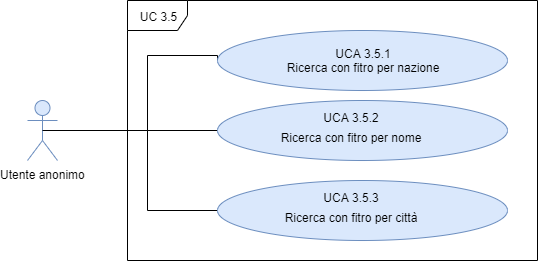
\includegraphics[scale=0.5]{sezioni/UseCase/Immagini/UCA3.5.png}
	\caption{UCA 3.5 - Ricerca personalizzata delle organizzazioni}
\end{figure}

\begin{itemize}
	\item \textbf{Attori primari:} Utente anonimo;
	\item \textbf{Precondizione:} L'utente è autenticato e può svolgere ricerche riguardo le organizzazioni;
	\item \textbf{Postcondizione:} Vengono forniti all'utente i risultati delle ricerche;
	\item \textbf{Scenario principale:} L'utente deve svolgere alcune ricerche e sceglie il metodo che più gli aggrada;
	\item \textbf{Flusso di eventi:} 
	\begin{itemize}
		%\item L'utente anonimo accede alla funzionalità "Ricerca personalizzata" della lista delle organizzazioni per ricercare le organizzazioni a cui interessa trovare
		\item UCA - 3.5.1 Ricerca per nazione;
		\item UCA - 3.5.2 Ricerca per nome;
		\item UCA - 3.5.3 Ricerca per città;
	\end{itemize}
	\item \textbf{Scenario alternativo:} Se non è presente nessuna lista delle organizzazioni viene visualizzato all'utente un messaggio di errore che lo informa di tale problema;
	\item \textbf{Estensioni:}
	\begin{enumerate}
		\item UCA 3.3.3 - Visualizzazione di un messaggio di errore che informa che non è salvata nessuna lista delle organizzazioni.
	\end{enumerate}
\end{itemize}

\subsubsection{UCA 3.5.1 - Ricerca per nazione}%fish level
\begin{itemize}
	\item \textbf{Attori primari:} Utente anonimo;
	\item \textbf{Precondizione:} L'utente anonimo può utilizzare la funzionalità di ricerca della lista per cercare le organizzazioni di una certa nazione d'interesse;
	\item \textbf{Postcondizione:} Viene visualizzato la lista delle organizzazioni che sono nella città scelta dall'utente.
\end{itemize}

\subsubsection{UCA 3.5.2 - Ricerca per nome}%fish level
\begin{itemize}
	\item \textbf{Attori primari:} Utente anonimo;
	\item \textbf{Precondizione:} L'utente anonimo può utilizzare la funzionalità di ricerca della lista per cercare il le organizzazioni che hanno il nome specificato dall'utente;
	\item \textbf{Postcondizione:} Viene visualizzato la lista delle organizzazioni che hanno il nome sceltao dall'utente.
\end{itemize}

\subsubsection{UCA 3.5.3 - Ricerca per città}%fish level
\begin{itemize}
	\item \textbf{Attori primari:} Utente anonimo;
	\item \textbf{Precondizione:} L'utente anonimo può utilizzare la funzionalità di ricerca della lista per cercare il le organizzazioni di una certa città d'interesse;
	\item \textbf{Postcondizione:} Viene visualizzato la lista delle organizzazioni che sono nella nazione scelta dall'utente.
\end{itemize}

